\documentclass[border=4pt,12pt]{standalone}
% House style for redrawn exam diagrams (diagram-v4: 0.4pt lines, filled -latex arrows, fine dashes; stipple and hatching drawn as real dots/lines (no PDF/SVG patterns, so they render in every browser and at any scale); transparent background). Every figure \input's this.
\usepackage{amsmath,amssymb}
\usepackage{txfonts}
\usepackage{pdfrender,xcolor}
% \halo{text}: label on shading. The shading stops just around each letter's outline (a thin knock-out that follows the
% glyphs, like the papers' typesetting), never a box. Owner: "I don't want a box around the text".
\newcommand{\halo}[1]{\leavevmode\rlap{\pdfrender{TextRenderingMode=2,LineWidth=2.2pt,LineJoinStyle=1,StrokeColor=white,FillColor=white}#1}#1}
\usepackage{tikz,pgfplots}
\pgfplotsset{compat=1.18}
\usetikzlibrary{arrows.meta,calc,angles,quotes,patterns,patterns.meta,intersections,positioning,decorations.markings,shapes.geometric}
% Stipple and hatching are drawn as actual dots / lines clipped to the region (path picture), NOT as pattern fills:
% SVG <pattern> fills vanish or blur when browsers scale the image, so the owner could not see the shading.
% Each dot is a 0.72pt square (keeps SVGs small; reads as a dot at print size). Dots sit on one global staggered grid, so neighbouring regions line up.
\makeatletter
\newdimen\ex@x \newdimen\ex@y \newdimen\ex@xa \newdimen\ex@ya \newdimen\ex@xb \newdimen\ex@yb \newcount\ex@row
\def\exam@stipplecolor{black!75}\def\exam@dotr{0.42pt}\def\exam@dotgap{2.5}
\def\ex@rowdots{\ifdim\ex@x<\ex@xb \pgfpathrectangle{\pgfqpoint{\dimexpr\ex@x-0.36pt\relax}{\dimexpr\ex@y-0.36pt\relax}}{\pgfqpoint{0.72pt}{0.72pt}}\advance\ex@x by \exam@dotgap pt\relax\expandafter\ex@rowdots\fi}
\def\exam@stipple{%
  \pgftransformreset% dots are sized in real points even inside scaled pictures
  \pgfpointanchor{path picture bounding box}{south west}\ex@xa=\pgf@x \ex@ya=\pgf@y
  \pgfpointanchor{path picture bounding box}{north east}\ex@xb=\pgf@x \ex@yb=\pgf@y
  \pgfsetfillcolor{\exam@stipplecolor}\pgfmathsetmacro\ex@h{\exam@dotgap/2}%
  \pgfmathtruncatemacro\ex@r{floor(\ex@ya/\ex@h)-1}\ex@row=\ex@r\relax
  \ex@y=\ex@r\dimexpr\ex@h pt\relax
  \loop\ifdim\ex@y<\ex@yb
    \pgfmathtruncatemacro\ex@c{floor(\ex@xa/\exam@dotgap)-1}\ex@x=\ex@c\dimexpr\exam@dotgap pt\relax
    \ifodd\ex@row \advance\ex@x by \ex@h pt\fi
    \ex@rowdots
    \advance\ex@y by \ex@h pt \advance\ex@row by 1
    \ifnum\numexpr\ex@row-(\ex@row/4)*4\relax=0 \pgfusepath{fill}\fi% flush every 4 rows: bounded TeX memory, few clip copies in the SVG
  \repeat\pgfusepath{fill}}
\newdimen\ex@d
\def\exam@hatch#1{% #1 = 1 for /, -1 for \ ; lines 45 degrees, 3pt apart
  \pgftransformreset
  \pgfpointanchor{path picture bounding box}{south west}\ex@xa=\pgf@x \ex@ya=\pgf@y
  \pgfpointanchor{path picture bounding box}{north east}\ex@xb=\pgf@x \ex@yb=\pgf@y
  \ex@d=\dimexpr\ex@yb-\ex@ya\relax \ex@x=\dimexpr\ex@xa-\ex@d\relax
  \loop\ifdim\ex@x<\ex@xb
    \ifnum#1>0 \pgfpathmoveto{\pgfqpoint{\ex@x}{\ex@ya}}\pgfpathlineto{\pgfqpoint{\dimexpr\ex@x+\ex@d\relax}{\ex@yb}}%
    \else \pgfpathmoveto{\pgfqpoint{\ex@x}{\ex@yb}}\pgfpathlineto{\pgfqpoint{\dimexpr\ex@x+\ex@d\relax}{\ex@ya}}\fi
    \advance\ex@x by 4.24pt
  \repeat
  \pgfsetlinewidth{0.4pt}\pgfsetstrokecolor{black}\pgfusepath{stroke}}
\def\examstipple{\exam@stipple}\def\examhatch{\exam@hatch}\def\examsetstipplecolor#1{\def\exam@stipplecolor{#1}}\def\examsetdotgap#1{\def\exam@dotgap{#1}}
\makeatother
% (legacy pattern kept for old files)
% staggered stipple like the NESA papers' dotted shading
\pgfdeclarepatternformonly{exam stipple}{\pgfpointorigin}{\pgfqpoint{2.2pt}{2.2pt}}{\pgfqpoint{2.2pt}{2.2pt}}{%
  \pgfpathcircle{\pgfqpoint{0.55pt}{0.55pt}}{0.42pt}\pgfpathcircle{\pgfqpoint{1.65pt}{1.65pt}}{0.42pt}\pgfusepath{fill}}
\tikzset{
  every picture/.style={line width=0.6pt, >={Latex[length=2mm,width=1.3mm]}},
  curve/.style={line width=0.6pt},
  open arrow/.style={-{Latex[length=2mm,width=1.3mm]}},  % owner: filled -latex heads everywhere, no open chevrons
  aux/.style={dash pattern=on 2pt off 1.5pt, line width=0.6pt},
  shade/.code={\def\exA{#1}\def\exB{none}\ifx\exA\exB\else\pgfkeysalso{fill=black!18}\fi},
  shade/.default=on,
  shade dots/.style={fill=none, path picture={\examstipple}},
  stipple color/.code={\examsetstipplecolor{#1}},
  stipple gap/.code={\examsetdotgap{#1}},
  shade dense dots/.style={fill=none, stipple gap=1.6, path picture={\examstipple}},
  shade hatch/.style={fill=none, path picture={\examhatch{1}}},
  shade hatch reverse/.style={fill=none, path picture={\examhatch{-1}}},
  shade solid/.style={fill=black},
  pt/.style={circle, fill, inner sep=1.1pt},
  open pt/.style={circle, draw, fill=white, inner sep=1.1pt},
}
\pgfplotsset{
  exam axes/.style={axis lines=middle, axis line style={->}, xlabel={$x$}, ylabel={$y$},
    xlabel style={anchor=west}, ylabel style={anchor=south}, tick label style={font=\small},
    every axis plot/.append style={line width=0.6pt, black}, samples=200, clip=false,
    enlargelimits=false, axis on top},
}

\begin{document}
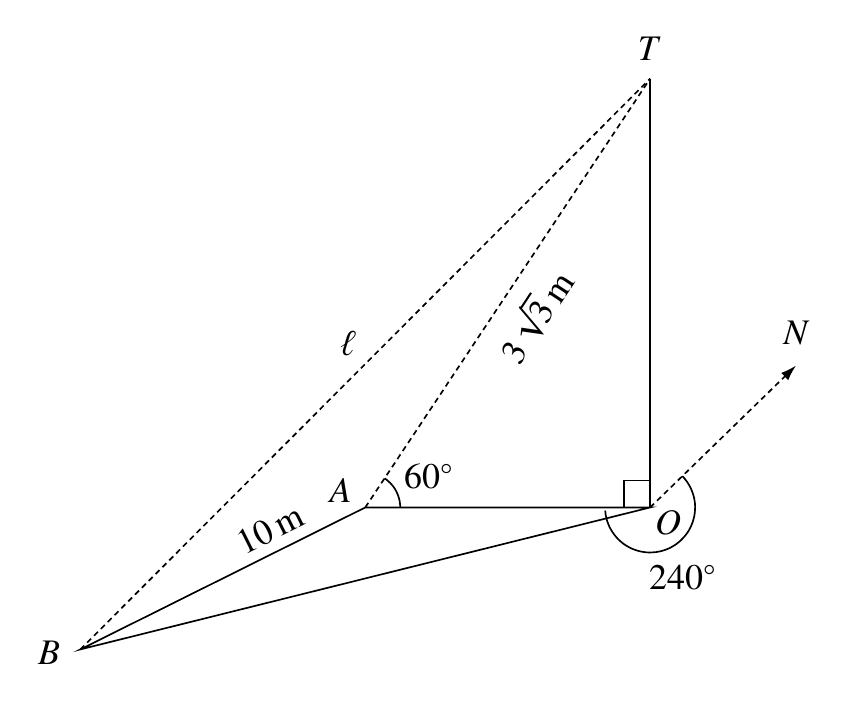
\begin{tikzpicture}[x=0.0127cm,y=-0.0127cm, every node/.style={font=\fontsize{13}{15}\selectfont}]
\draw (632,487) -- (632,58);
\draw (347,487) -- (632,487) -- (62,629) -- cycle;
\draw[aux] (62,629) -- (632,58);
\draw[aux] (347,487) -- (632,58);
\draw[aux,->] (632,487) -- (778,345);
\draw (606,487) -- (606,460) -- (632,460);
\draw plot[smooth] coordinates {(382.0,487.0) (382.0,485.2) (381.8,483.4) (381.6,481.6) (381.3,479.8) (380.8,478.0) (380.3,476.3) (379.7,474.6) (379.0,472.9) (378.3,471.3) (377.4,469.7) (376.5,468.1) (375.5,466.6) (374.4,465.2) (373.2,463.8) (372.0,462.5) (370.6,461.2) (369.3,460.0) (367.9,458.9) (366.4,457.8)};
\draw plot[smooth] coordinates {(664.3,455.6) (665.6,457.0) (666.8,458.5) (668.0,460.1) (669.2,461.6) (670.2,463.3) (671.2,464.9) (672.1,466.7) (673.0,468.4) (673.7,470.2) (674.4,472.0) (675.0,473.9) (675.6,475.7) (676.0,477.6) (676.4,479.5) (676.7,481.4) (676.9,483.4) (677.0,485.3) (677.0,487.3) (676.9,489.2) (676.8,491.1) (676.6,493.1) (676.3,495.0) (675.9,496.9) (675.4,498.8) (674.9,500.6) (674.3,502.5) (673.5,504.3) (672.8,506.1) (671.9,507.8) (671.0,509.5) (670.0,511.2) (668.9,512.8) (667.7,514.4) (666.5,515.9) (665.2,517.3) (663.9,518.7) (662.5,520.1) (661.0,521.4) (659.5,522.6) (658.0,523.8) (656.4,524.8) (654.7,525.9) (653.0,526.8) (651.3,527.7) (649.5,528.5) (647.7,529.2) (645.8,529.8) (644.0,530.4) (642.1,530.9) (640.2,531.2) (638.3,531.6) (636.3,531.8) (634.4,531.9) (632.5,532.0) (630.5,532.0) (628.6,531.9) (626.7,531.7) (624.7,531.4) (622.8,531.1) (620.9,530.6) (619.1,530.1) (617.2,529.5) (615.4,528.8) (613.6,528.1) (611.8,527.2) (610.1,526.3) (608.4,525.3) (606.8,524.3) (605.2,523.2) (603.7,522.0) (602.2,520.7) (600.8,519.4) (599.4,518.0) (598.1,516.6) (596.9,515.1) (595.7,513.6) (594.6,512.0) (593.5,510.3) (592.5,508.6) (591.6,506.9) (590.8,505.2) (590.1,503.4) (589.4,501.5) (588.8,499.7) (588.3,497.8) (587.9,495.9) (587.5,494.0) (587.3,492.1) (587.1,490.1)};
\node at (632,28) {$T$};
\node at (778,313) {$N$};
\node at (330,323) {$\ell$};
\node[rotate=56.4] at (517,295) {$3\sqrt{3}\,\mathrm{m}$};
\node at (411,456) {$60^\circ$};
\node at (322,470) {$A$};
\node[rotate=26.5] at (252,509) {$10\,\mathrm{m}$};
\node at (650,503) {$O$};
\node at (665,557) {$240^\circ$};
\node at (30,632) {$B$};
\end{tikzpicture}
\end{document}